\documentclass[11pt]{article}
\usepackage[margin=1in]{geometry}
\usepackage{graphicx}
\usepackage{amsmath,amssymb}
\usepackage{booktabs}
\usepackage{xcolor}
\usepackage{caption}
\usepackage{subcaption}
\usepackage[colorlinks=true,linkcolor=blue,citecolor=blue,urlcolor=blue]{hyperref}
\graphicspath{{../figures/}}

\title{\textbf{Learning to Drive a Single Go1 Quadruped to a Target\\
from Any Position: Offline RL and PPO on Real Motion-Capture Data}}
\author{EKF Physical RL project --- \texttt{realdata/real\_model\_v1}}
\date{\today}

\begin{document}
\maketitle

\begin{abstract}
We learn a control policy that drives a \emph{single} Unitree Go1 quadruped from
\emph{any} start position inside a fixed arena to the target
$\mathbf g=(-2.0,-2.5)\,$m, subject to a maximum-speed limit and a hard
requirement never to leave the map. The policy is grounded in $23$ real
motion-capture runs. We take great care with the data: each trajectory is
truncated at its first goal entry, a goal entry is the \emph{only} event that
counts as a terminal state, and each run is classified as reaching / approaching
/ non-reaching so that the one wandering run that never approaches the goal is
never treated as a successful demonstration. We compare three offline
off-policy algorithms (TD3+BC, IQL, CQL) trained on the real transitions with
PPO trained online in a data-grounded kinematic simulator. Evaluated from
$200$ random start positions across the whole map, all four reach the goal
$100\%$ of the time, but they differ sharply on the constraints: \textbf{PPO}
reaches with \textbf{zero boundary violations} and near-time-optimal paths,
whereas the offline methods reach the goal but graze the walls --- because the
real data never violates the boundary, an offline learner cannot see the
penalty that teaches avoidance. We release all policies, animations, and an
analysis of the $15{,}263$ onboard camera frames motivating a vision-based
extension.
\end{abstract}

\section{Task and World}
\textbf{Single agent.} There is one robot; all data are for that robot.
\textbf{Objective.} From any pose inside the arena, drive to the fixed goal
$\mathbf g=(-2.0,-2.5)\,$m and stop within $\rho=0.30\,$m of it, while
(i)~respecting a maximum speed and (ii)~never leaving the map.

\textbf{Map.} The arena is the rectangle
$[-2.15,2.00]\times[-2.70,2.40]\,$m, obtained by expanding the observed mocap
extent ($x\in[-1.94,1.84]$, $y\in[-2.54,2.26]$) so that it contains the goal,
which sits in the bottom-left corner.

\textbf{Speed limit.} From the data, the body linear speed has $99$th
percentile $\approx1.4\,$m/s and the yaw rate $\approx2.4\,$rad/s. We cap the
admissible action at $|(v_x,v_y)|\le V_{\max}=1.5\,$m/s and
$|\omega|\le W_{\max}=2.5\,$rad/s.

\section{Careful Data Handling}
Each mocap run is resampled to a uniform $10\,$Hz grid; yaw is taken from the
quaternion. We then, per run:
\begin{enumerate}\itemsep2pt
  \item classify it by how close it gets to the goal --- \textbf{REACH} (enters
  the $0.30\,$m radius), \textbf{approach} (net progress $>0.5\,$m but never
  enters), or \textbf{NON-REACH};
  \item \textbf{truncate at the first goal entry}, discarding post-goal drift so
  that lingering near the goal is not mislabelled;
  \item extract the action $a=(v_x,v_y,\omega)$ as the body-frame twist by
  finite differencing, then \textbf{clip it to the speed limit} (this also
  removes mocap spikes);
  \item set the terminal flag \textbf{true only at a genuine goal entry}. A run
  that merely stops is a \emph{truncation}, not a terminal state; treating it as
  terminal would wrongly cut the value bootstrap and corrupt learning.
\end{enumerate}
Of the $23$ runs, $17$ REACH, $5$ approach and $1$ is NON-REACH
(Fig.~\ref{fig:data}): run \texttt{20260624\_153602} starts $3.74\,$m from the
goal, wanders for $120\,$s and \emph{ends farther away} ($4.21\,$m, closest
approach $1.28\,$m). We keep it in the buffer for state-space coverage but,
because rewards are progress-based, its transitions receive correctly low
values, so value-based offline RL never imitates it. The final dataset has
$4{,}705$ transitions with $17$ true terminals.

\begin{figure}[t]
  \centering
  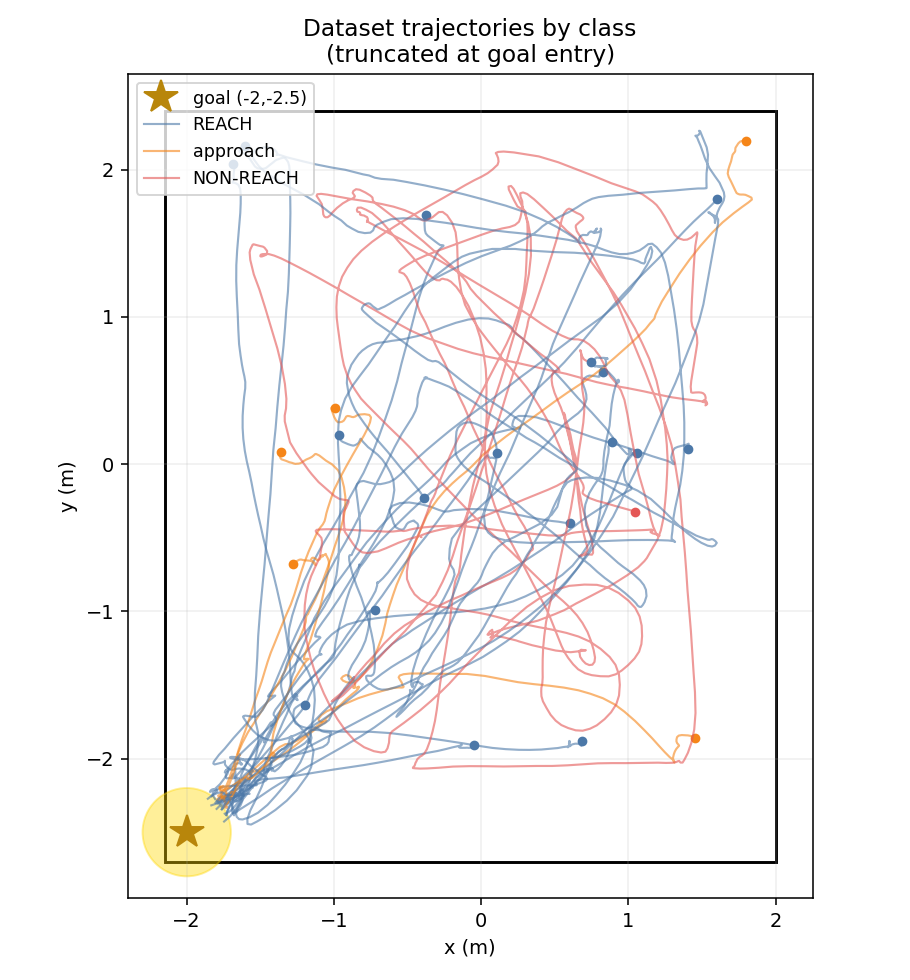
\includegraphics[width=0.55\linewidth]{dataset_classified.png}
  \caption{The $23$ runs coloured by class (truncated at goal entry). Blue
  REACH runs converge to the goal; the single red NON-REACH run wanders the
  arena and never approaches the corner --- it must not be treated as a
  successful demonstration.}
  \label{fig:data}
\end{figure}

\section{MDP and Environment}
\textbf{Observation (position-aware, 9-D).}
$s=[\,x,\,y,\,\cos\psi,\,\sin\psi,\,g^b_x,\,g^b_y,\,v_x,\,v_y,\,\omega\,]$, where
$(g^b_x,g^b_y)$ is the goal in the body frame. The absolute position $(x,y)$ is
included so the policy can reason about the walls (goal-relative features alone
cannot express where the boundary is).

\textbf{Action.} Body-frame twist $a=(v_x,v_y,\omega)$, clipped to the speed
limit inside the environment.

\textbf{Reward (designed).} With $d_t=\lVert\mathbf g-\mathbf p_t\rVert$,
\begin{equation}
r_t = 5\,(d_t-d_{t+1}) \;-\; 0.01\lVert a_t\rVert^2 \;-\; 0.02
      \;+\; 20\cdot\mathbb 1[d_{t+1}<\rho] \;-\; 5\cdot\mathbb 1[\text{wall}].
\end{equation}
The dense progress term drives goal-reaching; the terminal bonus sharpens the
stop; the wall term (active only when the robot pushes against a boundary)
teaches map-compliance.

\textbf{Environment.} First-order kinematic body-velocity dynamics --- the exact
inverse of the action extraction, so data and simulator are consistent. The
robot is hard-clamped inside the map (it \emph{cannot} leave), and pushing
against a wall incurs the penalty. Episodes reset to \textbf{random poses across
the whole map}, which is what makes the learned policy work from any position.

\section{Algorithms}
Three \emph{offline} off-policy methods learn from the real transitions:
\textbf{TD3+BC}, \textbf{IQL} (expectile $0.7$, AWR temperature $3.0$),
\textbf{CQL} (SAC backbone, conservative penalty). \textbf{PPO} is
\emph{on-policy}, so it cannot consume the offline data directly; instead it
trains online in the data-grounded environment, where it sees the boundary
penalty and random starts. All share $2{\times}256$ MLPs, $\gamma=0.99$ and a
best-checkpoint rule that ranks by (success, then fewest wall violations, then
final distance).

\section{Results}
Every method is evaluated from the \emph{same} $200$ random start positions
across the map (Table~\ref{tab:res}, Figs.~\ref{fig:curves}--\ref{fig:anim}).

\begin{table}[h]
\centering
\caption{Evaluation from 200 random map positions (best checkpoint). Wall-viol.
= fraction of episodes with boundary contact away from the cornered goal; path
ratio = path length / straight-line distance ($1$ is optimal).}
\label{tab:res}
\begin{tabular}{lccccc}
\toprule
Method & Success & Wall-viol.\ & Steps to goal & Path ratio & Type\\
\midrule
\textbf{PPO (winner)} & \textbf{1.00} & \textbf{0.00} & \textbf{21} & \textbf{0.93} & online in sim\\
IQL   & 1.00 & 0.17 & 66 & 1.34 & offline\\
TD3+BC & 1.00 & 0.47 & 34 & 1.01 & offline\\
CQL   & 1.00 & 0.94 & 66 & 2.41 & offline\\
\bottomrule
\end{tabular}
\end{table}

All four reach the goal from any position, so the \emph{go-to-goal} objective is
solved by every method. The decisive differences are the \emph{constraints}:
PPO never touches a wall and takes essentially time-optimal, $\sim\!2\,$s paths
at near-maximum speed, while the offline methods --- which never observe a
boundary violation in the real data --- reach the goal but graze the walls
(CQL badly so). This is exactly why an \emph{online} learner in the
data-grounded simulator is the right tool for the ``from any position, stay in
the map'' requirement, with the offline policies serving as strong
data-driven baselines. The winning policy is saved to
\texttt{policies/best\_policy.pt}.

\begin{figure}[t]
  \centering
  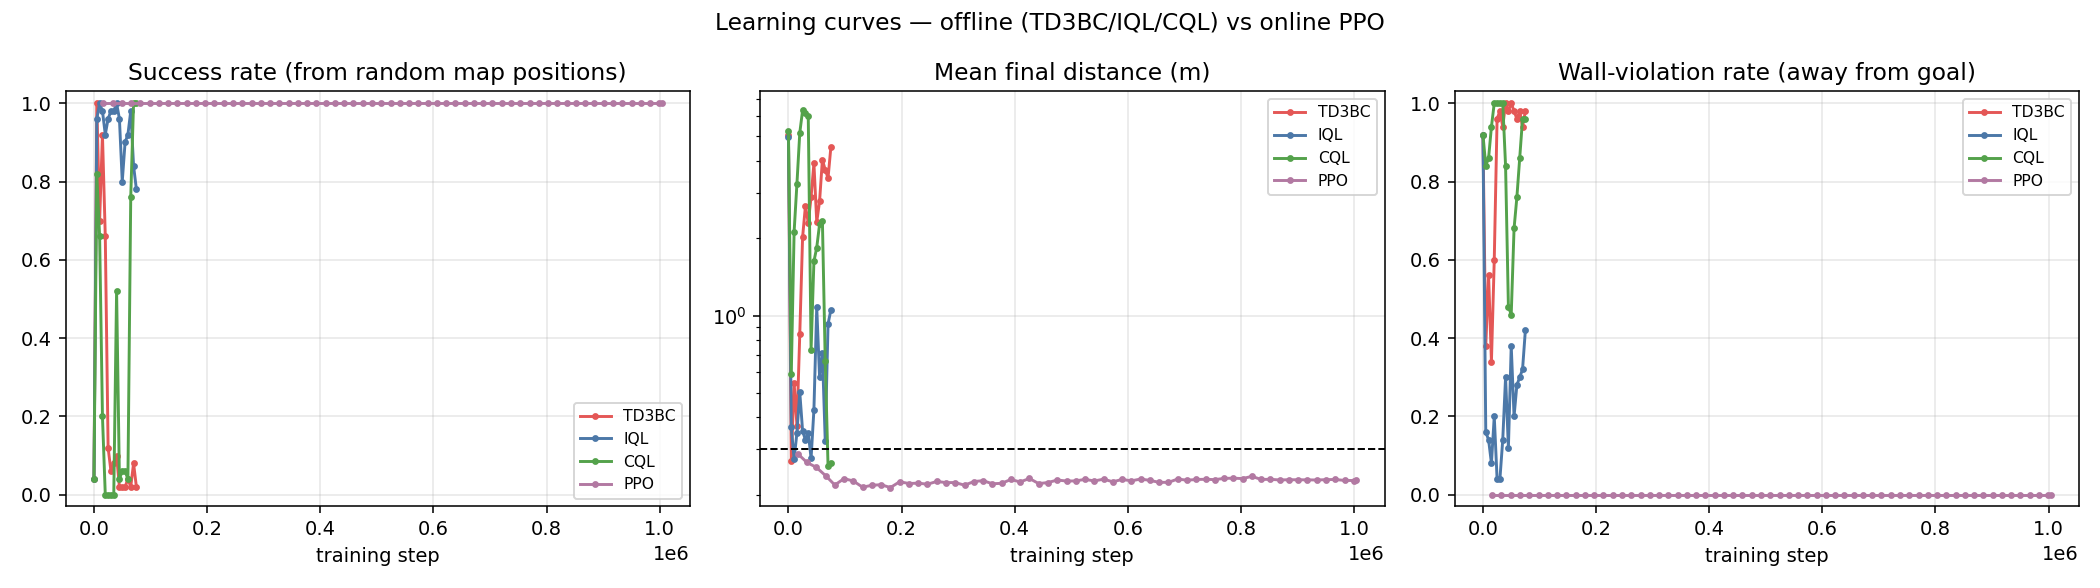
\includegraphics[width=0.99\linewidth]{learning_curves.png}
  \caption{Learning curves (evaluated from random map positions). PPO reaches
  $100\%$ success with a $0$ wall-violation rate; the offline methods reach the
  goal but retain higher wall-violation rates; TD3+BC and CQL are less stable.}
  \label{fig:curves}
\end{figure}

\begin{figure}[t]
  \centering
  \begin{subfigure}{0.42\linewidth}
    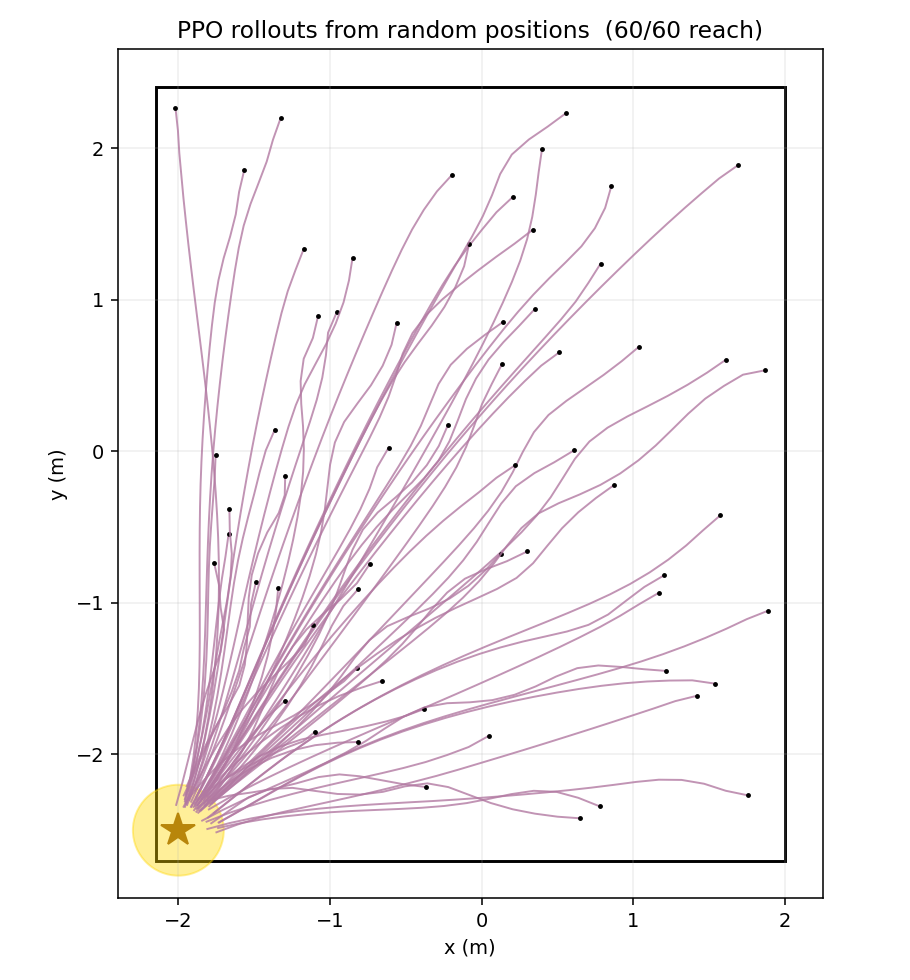
\includegraphics[width=\linewidth]{rollouts_PPO.png}
    \caption{PPO reaches from all random starts, inside the map.}
  \end{subfigure}\hfill
  \begin{subfigure}{0.56\linewidth}
    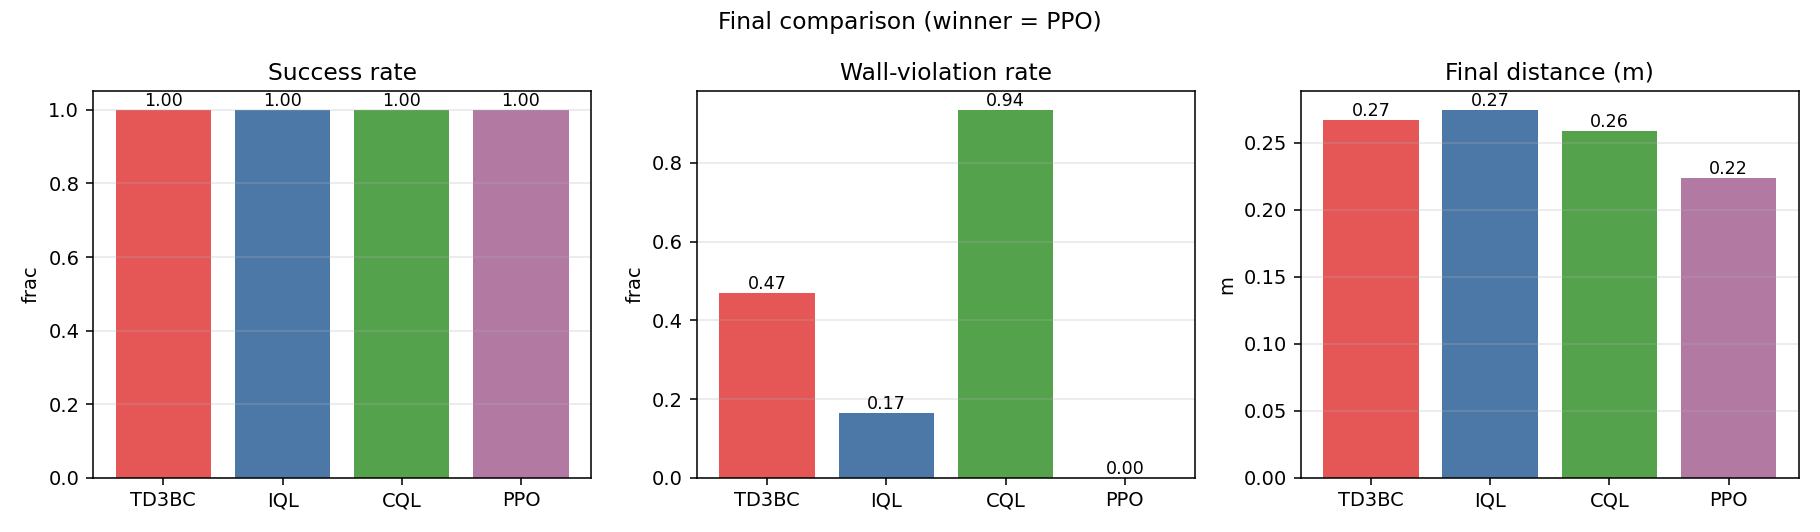
\includegraphics[width=\linewidth]{comparison_bar.png}
    \caption{Final metric comparison.}
  \end{subfigure}
  \caption{Winner behaviour and comparison. The black rectangle is the map
  boundary; the gold star/disc is the goal and its success radius.}
  \label{fig:rollouts}
\end{figure}

\begin{figure}[t]
  \centering
  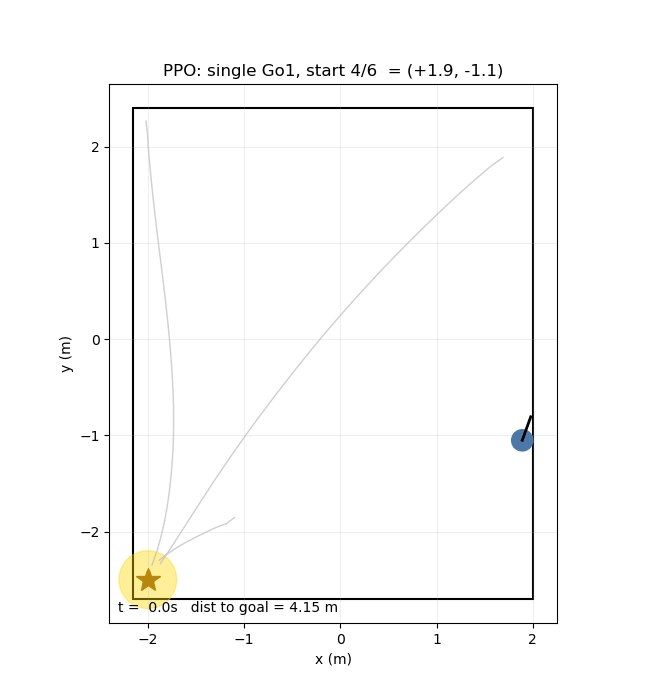
\includegraphics[width=0.5\linewidth]{anim_still_single_agent.png}
  \caption{Frame of \texttt{animations/single\_agent\_multistart.gif}: a
  \emph{single} Go1 (blue, with heading segment) driving to the goal, run from
  several different start positions \emph{in sequence}. Faded grey curves are the
  robot's earlier completed runs, illustrating that one policy reaches from
  anywhere in the map.}
  \label{fig:anim}
\end{figure}

\clearpage
\section{Onboard Camera Data: a Vision-Based Extension}
The policy uses only mocap pose, but the dataset also holds $15{,}263$ unused
onboard fisheye frames ($480\times400$; mean brightness $71.4$, mean Laplacian
sharpness $222.8$). Simple operators already expose task-relevant structure
(Fig.~\ref{fig:img}): walls and a doorway, stacked cardboard boxes that act as
obstacles, and floor markings.

\begin{figure}[h]
  \centering
  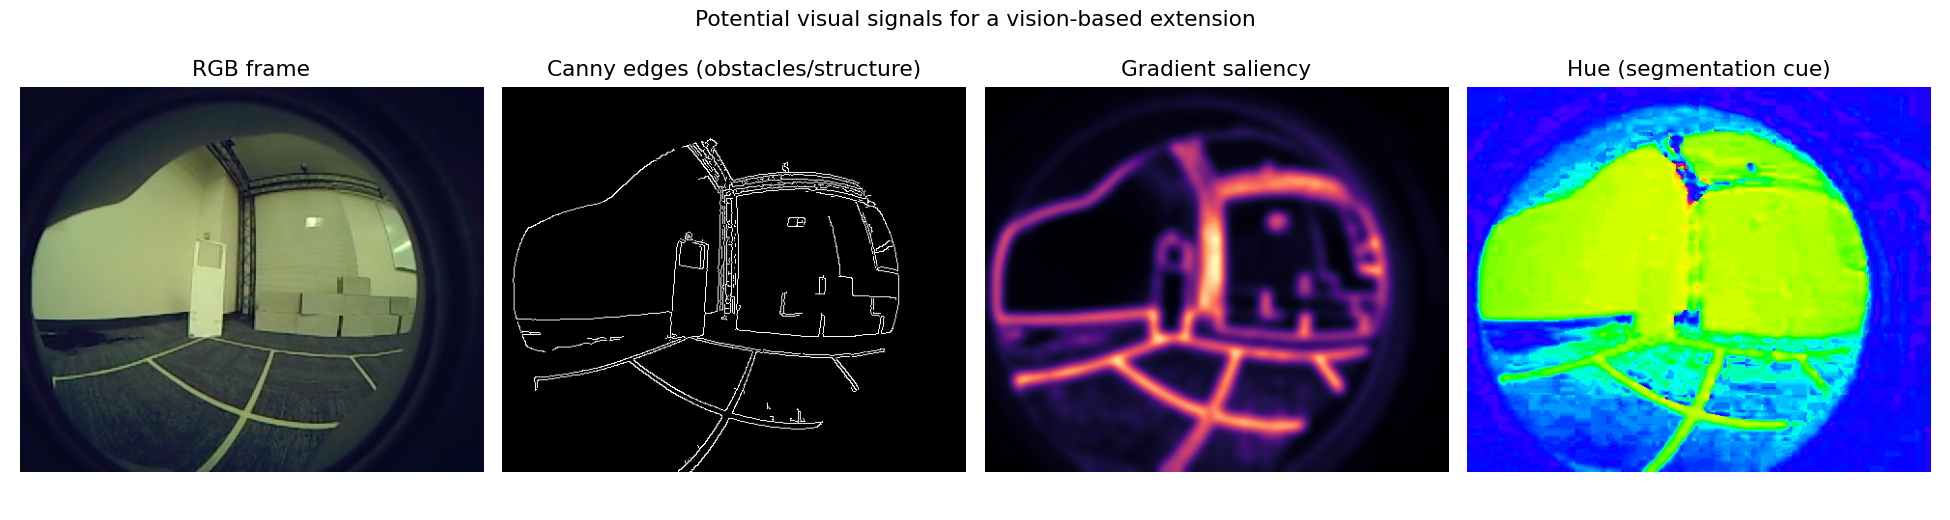
\includegraphics[width=0.99\linewidth]{img_potential.png}\\[3pt]
  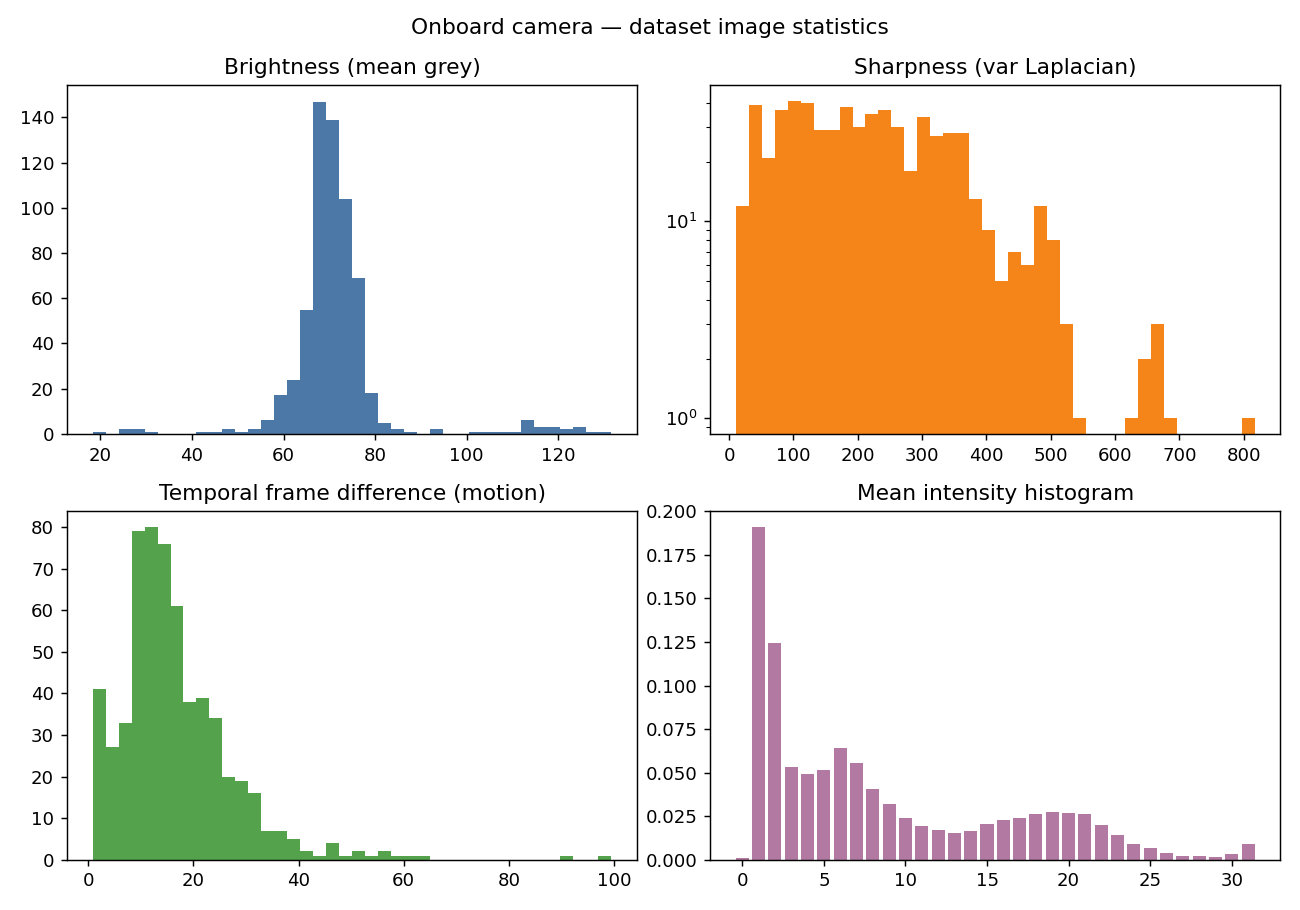
\includegraphics[width=0.78\linewidth]{img_stats.png}
  \caption{Top: a frame with edge / saliency / hue cues exposing obstacles,
  free space and structure. Bottom: dataset-wide image statistics.}
  \label{fig:img}
\end{figure}

\paragraph{Proposed extensions.}
(1)~\textbf{Vision-conditioned goal-reaching}: replace the mocap position with a
small CNN encoder, enabling deployment \emph{without} an external mocap system.
(2)~\textbf{Obstacle-aware navigation}: the visible boxes support a learned
collision-avoidance term, complementing the current wall constraint.
(3)~\textbf{Visual-inertial estimation}: fuse the camera with the logged
joint/IMU streams (the parent project's ``EKF'' theme) to recover pose when
mocap is unavailable. (4)~\textbf{Representation pretraining}: the $15$k frames
support self-supervised temporal-contrastive pretraining (mean inter-frame
difference $16.6$ confirms substantial motion) to warm-start the encoder.
Caveats visible in the data: strong fisheye distortion (calibrate/undistort)
and brightness varying $18$--$132$ across runs (photometric augmentation).

\section{Deliverables and Reproducibility}
The trained models live in a labeled \texttt{models/} folder: one subfolder per
model (\texttt{ppo\_online/}, \texttt{iql\_offline/}, \texttt{td3bc\_offline/},
\texttt{cql\_offline/}), each with its weights, \texttt{metrics.json} and a
detailed \texttt{model\_card.md}; the deployed winner is copied to
\texttt{models/best/}, and \texttt{models/MODELS.md} indexes them.

Pipeline: \texttt{python -m src.data\_pipeline} (build data) $\to$
\texttt{python -m src.train} (train the four methods, compare, save best) $\to$
\texttt{python -m src.export\_models} (labeled \texttt{models/} folder) $\to$
\texttt{python -m src.visualize} (figures + single-agent animation) $\to$
\texttt{python -m src.image\_analysis}. All runs use the \texttt{marl\_env}
conda env (PyTorch~2.7 + CUDA, RTX~4090) and a fixed seed; hyper-parameters are
in \texttt{src/config.py}.

\end{document}
